\chapter{Introduction}
\label{c1}

Artificial intelligence~(\as{ai}) has been widely embraced in our daily lives to help solving diverse tasks. \as{ai} is associated with giving machines the intelligence and ability to perform tasks or functions that would require human intelligence.
Specific examples of the use of \as{ai} include poetry writing, image generation, car driving, medical diagnosis, and playing strategic games \parencite{russell2009a}.

Natural language processing (\as{nlp}) is a subfield of \as{ai} that is related with making machines able to `understand' and communicate in human natural language, or simply perform processing of text \parencite{jurafsky2008a,indurkhya2010a}.
It has many applications ranging from more simple tasks, such as sentence boundaries detection and text classification, to more complex tasks including text summarization, question answering, and machine translation.
Using computers to automatically process text eases the analysis of large amounts of textual data.

Text data mining (\as{tdm}), or simply text mining (\as{tm}), involves the use of \as{nlp} methods to find new information from raw-text sources \parencite{hearst1999a,hotho2005a,allahyari2017a}.
\textcite{hearst1999a} argues that \as{tdm} makes use of text to directly discover heretofore unknown information.
The author refers an example where text can be used to form hypotheses for causes of rare diseases.
Information extraction~(\as{ie}) is the process of creating structured information, for example saved in the form of a database, from unstructured data.
As stated by \textcite{grishman2015a}, \as{nlp} researchers commonly refer to text as \textit{unstructured data}. However, in fact, natural language text has structure but it is not explicit---it is the goal of \as{ie} to make the text's semantic structure explicit.
More precisely, in the particular case of textual data, \as{ie} encompasses the identification of relationships and their arguments \parencite{grishman1997a,sarawagi2008a,grishman2019a}.
This is related with \as{tdm} since new knowledge can be unearthed and inferred from automatically extracted relationships between specific concepts mentioned in text. For instance in the biomedical domain this could mean to find interactions between concepts such as genes, diseases, chemical compounds, and food items.

\textcite{hearst1999a} also highlights the difference between information retrieval (or information access) and \as{tdm}. The former aims to help users find relevant documents (full-text or excerpts) according to their information needs \parencite{baezayates1999a}, while the goal of the latter is to derive or discover new information from free text (for example, finding previously unnoticed patterns across several datasets).

In this work we investigate the use of \as{nlp} and machine learning methods for expediting \as{ie} in the biomedical domain.
Large amounts of biomedical information, found in the life-sciences scientific literature and clinical narratives from electronic health records, are recorded in natural language text.
Therefore, it is imperative to use automatic \as{ie} solutions that can create structured information, from this vast data, for further use by \as{tdm} approaches to discover new knowledge---it is inconceivable for an individual to read and interpret all this textual data.

We consider that biomedical \as{ie} comprises two major tasks: (1) named entity recognition (\as{ner}), which is responsible for identifying biomedical entities in free text (such as genes and chemicals); and (2) relation extraction (\as{re}) which aims to determine biomedical relations between the previously recognized entities (such as protein--protein interactions).
Nevertheless, biomedical \as{ie} can benefit from other \as{nlp} tasks.
For instance, word sense disambiguation (\as{wsd}) aims to identify the proper meaning of an ambiguous term which is relevant to accurately define target entities.
Another task is document triage---its goal is to rank or classify documents according to their importance given a pre-defined criterion. For example, it could be used to find relevant documents for extracting specific biomedical interactions.


\section{Motivation}

Much of the biological, medical, and clinical knowledge is recorded in natural language form.
This textual data contains hidden relationships that can be exposed by automatic means, helping researchers to investigate new hypotheses that may contribute to a better health and well-being (for example, by finding potential treatments for specific diseases).

In the life sciences field the number of publications is increasingly high and it is hard for the interested audience---medical researchers, physicians, pharmacologists, and others---to keep up with the most recent research.
\Cref{fig:medline} shows an exponential growth of the number of publications indexed in \as{medline}, the leading biomedical bibliographic database compiled by the National Library of Medicine (\as{nlm}) of the United States.
We see that in the last years, more than 800~thousand scientific articles have been published per year.
The \as{covid19} epidemic~\parencite{velavan2020a} is a recent example showing that automatic methods are of utmost importance: they help specialists finding more appropriate resolutions for health problems.

Despite the undeniable value of biomedical free text present in scientific literature and clinical reports, the automatic processing of this type of text poses additional challenges when compared to text of the general domain.
For example, the biomedical vocabulary is regularly updated with new terms from novel discovered concepts, many terms have distinct meanings within different contexts, and the use of abbreviations further accentuates this ambiguity.
In the case of clinical text, this is even more difficult because abbreviations and typographical errors are more frequent.

The summarized aim of this work is to investigate the use of computer-based methods to extract relevant structured information from free text found in biomedical scientific literature and electronic health records.

% \FloatBarrier
\begin{figure}[!tb]
\begin{center}
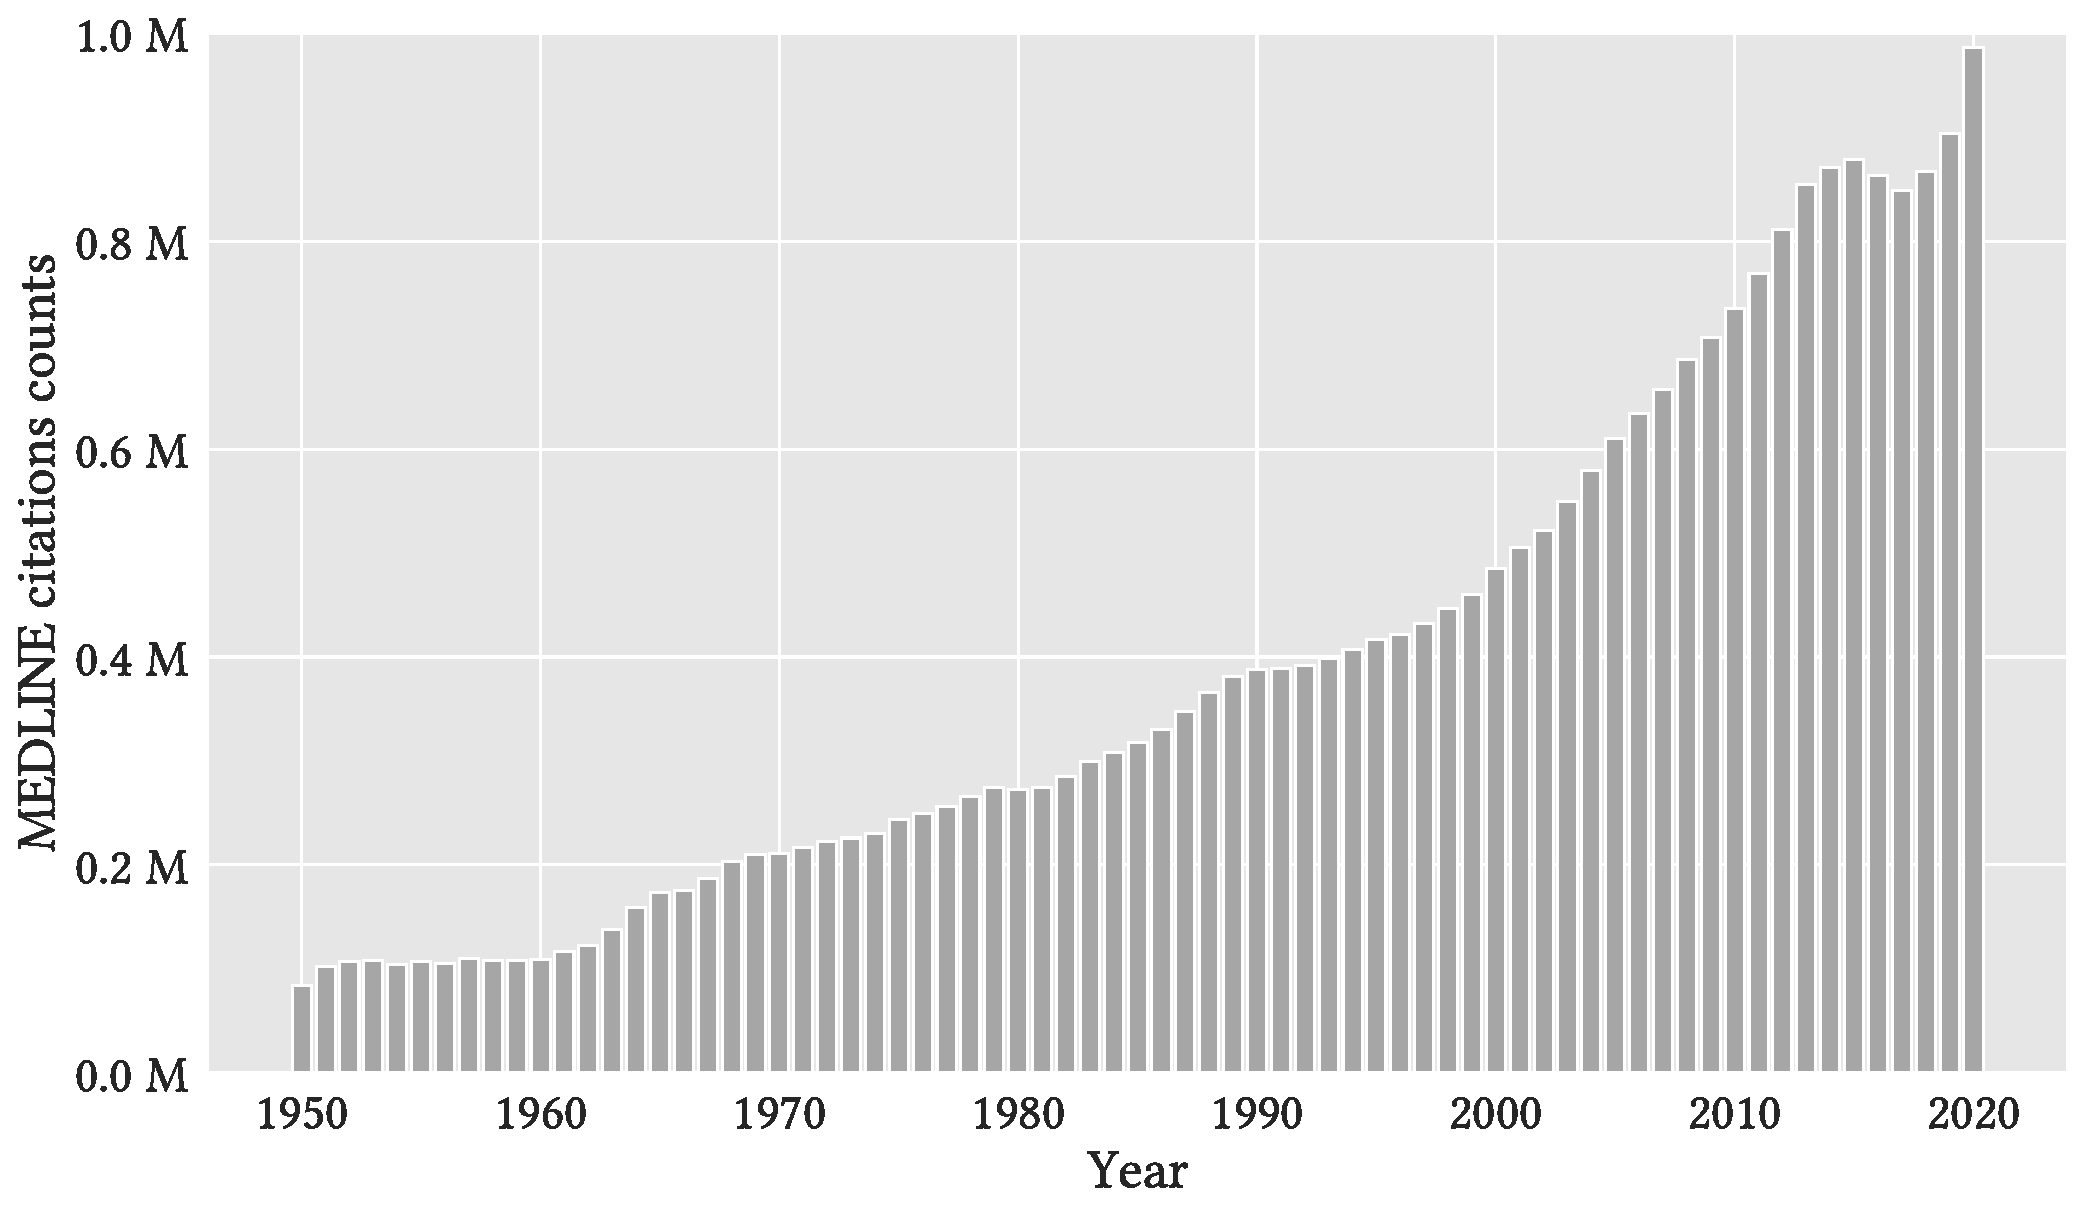
\includegraphics[width=\textwidth]{img/medline/v2/img.pdf}
\caption[Number of \as{medline} indexed publications by year of publication.]{Number of \as{medline} indexed publications by year of publication from 1950 to 2020 (as of January 2022). Data retrieved from \url{https://www.nlm.nih.gov/bsd/medline_cit_counts_yr_pub.html}.}
\label{fig:medline}
\end{center}
\end{figure}
% \FloatBarrier



\section{Thesis structure}

The remainder of this thesis is divided into five chapters.
A short description of each chapter follows.
Additionally, the rest of this first chapter contains a list of our publications, a description of our open-source contributions, and clarifications about the document design.

\settowidth{\mywidth}{\textbf{Chapter X}}
\begin{enumerate}[%
wide=0pt,%
labelwidth=\mywidth,
labelsep=5mm,%
leftmargin=\dimexpr\labelwidth+\labelsep\relax,%
]

\needspace{2\baselineskip}
\item[\textbf{Chapter 2}]
\textbf{Preliminaries}\newline
We present the fundamental notions of biomedical \as{nlp}, some biomedical resources, and the evaluation metrics commonly employed to compare the performance of \as{nlp} systems.
We explain in detail how \as{nlp} is used to process text, and how text is represented to be used by mathematical models.
We give emphasis to the biomedical \as{ie} task, explaining its components, and what methods and paradigms are usually considered.

\needspace{2\baselineskip}
\item[\textbf{Chapter 3}]
\textbf{Biomedical concept disambiguation}\newline
We enunciate related work describing automatic methods for disambiguation and normalization of biomedical terms in raw text.
We describe two different approaches for performing biomedical~\as{wsd}: supervised machine learning and knowledge-based.
We use bag-of-words, word embeddings, and different weighting schemes for representing the texts, showing how these are effective for this task.
In addition, we tackle the problem of normalization where we present a model based on word embeddings for linking clinical terms to standard vocabularies.

\needspace{2\baselineskip}
\item[\textbf{Chapter 4}]
\textbf{Biomedical text classification and similarity measurement}\newline
We justify, supported by background work, how text classification is relevant to \as{ie} and how measures of text similarity are significant for higher-level biomedical \as{nlp} applications.
We investigate the use of traditional machine learning classifiers, deep neural networks, and rule-based methods for text classification.
Lastly, we explore the application of deep learning, with word embeddings and sentence embeddings, for measuring semantic textual similarity.

\needspace{2\baselineskip}
\item[\textbf{Chapter 5}]
\textbf{Biomedical relation extraction}\newline
We describe related work on biomedical \as{re} from scientific literature and explain the task.
We present comprehensive experiments with convolutional and recurrent neural networks using word embeddings for identifying chemical--protein interactions~(\asp{cpi}) in biomedical scientific text, showing that neural networks methods perform competitively.

\needspace{2\baselineskip}
\item[\textbf{Chapter 6}]
\textbf{Conclusions}\newline
We discuss the overall work, highlight the main contributions, describe some limitations of our methods, and present future work directions.

\end{enumerate}


\section{Publications}

The work described here resulted in several publications.
A list of these, with a brief description, is presented chronologically by topic:

\begin{enumerate}[topsep=12pt,itemsep=12pt]

\item
\textbf{Machine learning with word embeddings applied to biomedical concept disambiguation} \parencite{antunes2016a}.\par
We apply traditional machine learning methods in a supervised setting for biomedical word sense disambiguation.
We combine bag-of-words and word embeddings to represent the surrounding textual context of ambiguous biomedical terms.
We compare word embedding models created from \as{pubmed} and Wikipedia, concluding that domain-specific biomedical word embeddings consistently provide better results.
\newline\textit{This publication is relevant to \Cref{c3}.}

\item
\textbf{Biomedical word sense disambiguation with word embeddings} \parencite{antunes2017a}.\par
We propose a knowledge-based method for biomedical word sense disambiguation.
We use the \as{umls} (Unified Medical Language System) and the \as{mesh} (Medical Subject Headings) term co-occurrences to extract concept textual definitions and calculate concept associations, respectively.
Each concept is represented by a vector weighted by the embeddings of the words in the concept definition.
We use word embedding models created from \as{pubmed} abstracts.
For disambiguation, cosine similarity is used to measure the similarity between the surrounding context of the ambiguous term and each possible concept.
We compare this knowledge-based method with machine learning methods using bag-of-words and word embeddings.
Despite being outperformed by machine learning methods, our proposed knowledge-based method achieves a comparable performance, does not require training data as in a supervised setting, and can be applied to any biomedical ambiguous term that contains a curated textual definition.
\newline\textit{This publication is relevant to \Cref{c3}.}

\item
\textbf{Evaluation of word embedding vector averaging functions for biomedical word sense disambiguation} \parencite{antunes2017b}.\par
We evaluate different word distance weighting schemes using our previously proposed knowledge-based method.
This weighting scheme is used to give more importance to the words closest to the ambiguous term.
We show that different weight schemes impact the disambiguation performance, and an adequate weighting can improve it.
\newline\textit{This publication is relevant to \Cref{c3}.}

\item
\textbf{Supervised learning and knowledge-based approaches applied to biomedical word sense disambiguation} \parencite{antunes2017c}.\par
One limitation of our biomedical \as{wsd} approach in past publications \parencite{antunes2017a,antunes2017b} was that we did not use the whole dataset for testing our knowledge-based method, because we did not have access to textual definitions for every concept in the dataset.
The main difference in this work is that we fetched textual definitions from \as{umls} for all concepts, enabling our results to be directly compared with other works in the literature.
This article presents an exhaustive compilation of experiments with different settings using supervised learning and knowledge-based systems.
We conclude that our knowledge-based method performs robustly, yet machine learning models provide higher performance but require labeled training data.
\newline\textit{This publication is relevant to \Cref{c3}.}

\item
\textbf{Clinical concept normalization on medical records using word embeddings and heuristics} \parencite{silva2020a}.\par
We employ sieve-based models (comprised of several steps)\footnote{Specifically, I was responsible for the first `sieve' of the model which was based on biomedical word embeddings for representing clinical terms.}, combined with heuristics and word embeddings, in clinical entity normalization.
This involves linking clinical named entities---such as drugs, disorders, and procedures---to concepts in established medical terminologies.
We show that the sole use of a strategy based on word embeddings presents competitive results.
\newline\textit{This publication is relevant to \Cref{c3}.}

\item
\textbf{Identifying relevant literature for precision medicine using deep neural networks} \parencite{matos2017a}.\par
We evaluate traditional classifiers against deep learning models for document classification, both using word embeddings, and show that deep neural network architectures obtain better results.
Our methods performed competitively in a document triage task,
which aimed to identify relevant \as{pubmed} abstracts that mention protein--protein interactions affected by genetic mutations.
\newline\textit{This publication is relevant to \Cref{c4}.}

\item
\textbf{Rule-based and machine learning hybrid system for patient cohort selection} \parencite{antunes2019a}.\par
We propose an automatic system to identify which patients, given their clinical textual reports, meet or not meet certain criteria (for example, does the patient uses drugs or speaks English).
The system is composed of rule-based methods with handcrafted text patterns and machine learning classifiers.
We show that some criteria are more easily solved with simple heuristics while others are more complex, demand specialized clinical knowledge for designing appropriate text patterns, and benefit from the use of machine learning models.
\newline\textit{This publication is relevant to \Cref{c4}.}

\item
\textbf{Evaluating semantic textual similarity in clinical sentences using deep learning and sentence embeddings} \parencite{antunes2020a}.\par
We present a deep neural network model for measuring the semantic similarity between clinical sentences.
In this task, a real value is attributed to each pair of sentences to specify the degree of the semantic meaning they share.
We assess the impact of using different pre-processing methods and feature representation methods (word embeddings against sentence embeddings).
\newline\textit{This publication is relevant to \Cref{c4}.}

\item
\textbf{Extraction of chemical--protein interactions from the literature using neural networks and narrow instance representation} \parencite{antunes2019b}.\par
We propose deep neural network models using word embeddings for extracting chemical--protein interactions from \as{pubmed} abstracts.
Our best model was based on recurrent neural networks and only used information from the shortest dependency path between the target entities.
We present an extensive study of experiments and make a detailed error analysis.
\newline\textit{This publication is relevant to \Cref{c5}.}

\end{enumerate}

Apart from the works summarized above, I colaborated in other works that are not discussed in this thesis.
These are presented in chronological order:

\begin{enumerate}

\item
Protein--protein interaction article classification using a convolutional recurrent neural network with pre-trained word embeddings \parencite{matos2017b}.

\item
Overview of the BioCreative VI Precision Medicine Track: mining protein interactions and mutations for precision medicine \parencite{dogan2019a}.

\item
Understanding depression from psycholinguistic patterns in social media texts \parencite{trifan2020a}.

\item
Machine learning for depression screening in online communities \parencite{trifan2020b}.

\item
Automatic analysis of artistic paintings using information-based measures \parencite{silva2021a}.

\item
Chemical--protein relation extraction in \as{pubmed} abstracts using \as{bert} and neural networks \parencite{antunes2021a}.

\item
Chemical detection and indexing in \as{pubmed} full text articles using deep learning and rule-based methods \parencite{almeida2021a}.

\item
Drug mention recognition in Twitter posts using a deep learning approach \parencite{silva2021b}.

\item
Chemical identification and indexing in PubMed full-text articles using deep learning and heuristics \parencite{almeida2022a}.

\item
Chemical identification and indexing in full-text articles: an overview of the \as{nlm}-Chem track at BioCreative VII \parencite{leaman2023a}.

\end{enumerate}


\section{Open-source contributions}

Some of the code developed for this thesis was made publicly available.
For that purpose, the following two open-source repositories were created:

\begin{itemize}

\item
\url{https://github.com/ruiantunes/2018-n2c2-track-1}\\
This repository contains part of the source code developed from our participation in the 2018~\as{n2c2} Track~1, comprising handcrafted rules and classical machine learning classifiers for automatic patient cohort selection \parencite{antunes2019a}.

\item
\url{https://github.com/ruiantunes/biocreative-vi-track-5-chemprot}\\
This repository contains the source code of our deep learning--based \as{re} extraction system for BioCreative~VI Track~5 integrating all post-challenge improvements \parencite{antunes2019b}.
We also share our word embedding models created from \as{pubmed} abstracts, and detailed statistics about the task dataset and our system predictions.

\end{itemize}


\section{Document writing and design}

Preparing a thesis document, that readers find comprehensible and compelling, is a challenging task.
As \textcite{zobel2014a} clarifies, the writing style must be adequate to communicate science: the text should be rigorous, readable, and based on logical thinking.
The author also presents a comprehensive discussion of many aspects of scientific writing, which I frequently consulted for improving the writing of this document.
Also relevant is a suitable design of the document by presenting its basic elements in an organized way. It makes the message of the author clearer, helping readers understanding it and keeping them interested \parencite{schriver1990a,telg2021a}.
It is difficult, if not impossible, to mention all the works that influenced and inspired me for better designing and structuring this document.
Still, I would like to point the reader to some major works that, in different ways, helped me to shape this document \parencite{oliveiraesilva1994a,campos2013a,gal2016a,baker2017a,amos2019a,oleynik2020a}.

The \LaTeX\ typesetting system was used to compose this document, and Inkscape was used for designing the vector images with the exception of \Cref{fig:medline} that was created using Matplotlib.
The source code for generating this thesis document is publicly available at:

\centerline{\url{https://github.com/ruiantunes/ua-thesis}.}
